%1) Relation complaint between customer and order and service employee
%2) Relation between order and customer (delivers)

\documentclass[12pt]{report}

\usepackage[utf8]{inputenc}
\usepackage{graphicx}

\graphicspath{..\ER Diagram}

\title{
    \textbf{Database Design for Online Retail Store\\ Winter 2022 \\}
}

\author{Abhimanyu Bhatnagar, 2020273
        \\Madhava Krishna, 2020217
        \\Ritika Nagar, 2020112
        \\Atyant Sony, 2020039}
\date{\textit{\today}}



\begin{document}
    \maketitle
    
    \tableofcontents
    \listoffigures
    \pagebreak

    %chapter 1, defining the problem
    \chapter{Defining the Problem}
    \section{Objective}
        The goal is to design a database management system for an online retail store,
        similar to Big Bazaar, Flipkart and Amazon. Our project models on Grofers (now BlinkIt), 
        a fast grocery marketplace for consumers to purchase day-to-day goods from.
    
    \section{Problem Statement}
    The ER diagrams and the relational schema that follow are based on the following (rudimentary) problem statement:
    \\\\
    %Problem statement
    \textit{
        The online retail store serves many customers. 
        The customers are required to hold an account on the platofrm to be able to purchase items.
        They can create an account by specifying their name, email address, phone number, and address.
        Customers add products to a shopping cart. They apply coupons on the shopping cart; the coupons 
        have a coupon code and an associated discount percentage.\\
        Customers order items by checking out the items on their shopping cart. The order is placed once the
         transaction is confirmed. The order is delivered to the customer only, 
         they cannot have the order delivered to other addresses.
        \\
        A product can belong to various categories and has specifications and a cost. Each
        product is obtained from a vendor which the store transacts with. After being purchased from 
        the vendor, the products are stored in a warehouse. Warehouse employees are responsible for packing 
        and preparing orders. The readied order is then delivered to the customer by a delivery agent.
        \\
        In case of any lapses with an order, the customer complains to support staff who create a complaint
        number against the order. They send out the details regarding the complaint to the customer.
    }

    \section{Stakeholders}
    Notable stakeholders of this problem include:
    \begin{enumerate}
        \item Customer
        \item Employees
        \item Suppliers
        \item Vendors
    \end{enumerate}
    Other stakeholders include manufacturers, warehousing service providers
    
    \section{Assumptions}
    \begin{enumerate}
        \item The retail store would be operated in one country only. Therefore, there isn't an option to change the country.
        \item There will be a shopping cart associated with the customer's account. They won't be able to add item to cart without being logged in.
        \item The delivery would be taken care of by the company itself; items will be shipped from one warehouse only (Similar to Blinkit, erstwhile Grofers).
        \item Coupons would be applied on the order, not the cart. Coupon would be applied during the checkout process.
        \item Coupons would be applied using the coupon code, which is a unique alphanumeric value. A coupon cannot be reused.
        \item Employees will be divided into delivery partners (responsible for delivering the order), warehouse workers (tasked with preparation of orders) and service employees (responsible for conflict resolution).
        \item Vendors have only one account number and will be based only in India.
        \item Employees have only one email address.
        \item There won't be any wishlisting features, nor any saved-items feature like the ones offered by Amazon.
        \item Employees' performance would be graded on a scale from 1 to 10 (for ease of data entry) with decimal values being permissible.
    \end{enumerate}



    \chapter{ER Diagram}
    
    \section{Entities}

    \begin{enumerate}
        \item Customer
            \begin{enumerate}
                \item \underline{Customer ID}: Primary key
                \item Phone Number: Multivalued
                \item Name: composite
                    \begin{enumerate}
                        \item First Name
                        \item Last Name
                    \end{enumerate}
                \item Address: composite
                    \begin{enumerate}
                        \item House Number
                        \item Locality
                        \item City
                        \item State
                        \item Pin Code
                    \end{enumerate}
                \item Email Address
                \item Password
            \end{enumerate}
        \item Product
            \begin{enumerate}
                \item \underline{Product ID}: Primary key
                \item Specifications
                    \begin{enumerate}
                        \item Expiry date
                        \item Manufacture date
                        \item Country of manufacture
                        \item Weight 
                        \item Dimensions
                    \end{enumerate}
                \item Price
                \item Category
                \item Discount Percentage
                \item GST
                \item Rating : Multivalued
                \item Photos: Multivalued
            \end{enumerate}
        \item Orders
            \begin{enumerate}
                \item \underline{Order ID}
                \item Cost of products
                \item Taxes
                \item Discount Percentage
            \end{enumerate}
        \item Vendor
            \begin{enumerate}
                \item \underline{Vendor ID}
                \item Address
                    \begin{enumerate}
                        \item Plot number
                        \item City
                        \item State
                        \item Pin code
                    \end{enumerate}
                \item Name
                \item Phone number
            \end{enumerate}
        \item Coupon
            \begin{enumerate}
                \item \underline{Coupon Code}: Primary key
                \item Discount Percentage
                \item Validity
            \end{enumerate}
        \item Warehouse
            \begin{enumerate}
                \item \underline{Warehouse ID}
                \item Address: composite
                    \begin{enumerate}
                        \item Plot number
                        \item City
                        \item State
                        \item Pin Code
                    \end{enumerate}
                \item Telephone Number: multivalued
            \end{enumerate}
        \item Employee:
            \begin{enumerate}
                \item \underline{Employee ID}: Primary key
                \item Date of Joining
                \item Position
                \item Department
                \item Email Address
                \item Name: composite
                    \begin{enumerate}
                        \item First Name
                        \item Last Name
                    \end{enumerate}
                \item Residential Address: composite
                    \begin{enumerate}
                        \item House number
                        \item Locality
                        \item City
                        \item State
                        \item Pin Code
                    \end{enumerate}
                \item Date of Joining
                \item Performance
                \item Salary
                \item Gender
                \item Date of Birth
                \item Age : derived
            \end{enumerate}
            Employees can be specialised into:
            \begin{itemize}
                \item Delivery Partner:
                    \begin{enumerate}
                        \item Vehicle ID
                        \item Vehicle Type
                    \end{enumerate}
                \item Warehouse Worker: no additional attributes
                \item Service Employee: no additional attributes
            \end{itemize}
        \item Shopping Cart (Weak entity)
            \begin{enumerate}
                \item \underline{Customer ID,Product ID}: Primary Key
                \item Customer ID: Foreign Key (references Customer)
                \item Product ID: Foreign Key (references Product)
                \item Quantity
                \item Total cost: Derived attribute

            \end{enumerate}
        
    \end{enumerate}


    \section{Relations}
        \begin{enumerate}
             \item Supplies: between vendor and product
            \begin{enumerate}
                \item \underline{Vendor ID, Product ID}: Primary Key
                \item Vendor ID: Foreign Key (references Vendor)
                \item Product ID: Foreign Key (references Product)
                \item Quantity: attribute
            \end{enumerate}
            \item Includes: between product and order to show which order contained what products
            \begin{enumerate}
                \item \underline{Order ID, Product ID}: Primary Key 
                \item Order ID: Foreign Key (references Order)
                \item Product ID: Foreign Key (references Product)
                \item Quantity: attribute
            \end{enumerate}
            \item Stores: between warehouse and product to show which warehouse contains what products.
            \begin{enumerate}
                \item \underline{Warehouse ID, Product ID}: Primary Key
                \item Warehouse ID: Foreign Key (references Warehouse)
                \item Product ID: Foreign Key (references Product)
                \item Stocks: attribute
            \end{enumerate}
            \item Delivery: Quarternary relation between warehouse, order, delivery partner and customer to represent delivery.
            \begin{enumerate}
                \item \underline{Order ID}: Primary Key
                \item Order ID: Foreign Key (references Order)
                \item Employee ID: Foreign Key (references Employee)
                \item Customer ID: Foreign Key (references Customer)
                \item Warehouse ID: Foreign Key (references Warehouse)
            \end{enumerate}
            \item Transaction: Relation between customer and their cart, order and coupon code.
            \begin{enumerate}
                \item \underline{Order ID}: Primary Key
                \item Customer ID: Foreign Key (references Customer)
                \item Payment Method
                \item Transaction Status
                \item Transaction Time
                \item Coupon Code: Foreign Key (references Coupon)
            \end{enumerate}
            \item Complains: between service employees (specialisation), customer and order to indicate a dispute.
            \begin{enumerate}
                \item \underline {Complaint Number}: Primary Key
                \item Customer ID: Foreign Key (references Customer)
                \item Order ID: Foreign Key (references Order)
                \item Service Employee ID: Foreign Key (references Employee)
            \end{enumerate}
	\item Works in: between Warehouse Worker and warehouse.
	\begin{enumerate}
				\item \underline{Employee ID, Warehouse ID}: Primary key
			\end{enumerate}
	\item Has: relation between customer and shopping cart (weak entity).
			\begin{enumerate}
				\item \underline{Customer ID}: Primary key
			\end{enumerate}
	\item Contains: relation between shopping cart and product to indicate that shopping cart contains the item.
		\begin{enumerate}
			\item Quantity
			\item Cost of items in the cart: Derived quantity.
		\end{enumerate}
	\item Rates: between customer and product for indicating rating.
		\begin{enumerate}
			\item \underline{Customer ID, Product ID}: Primary key
			\item Rating: attribute
		\end{enumerate}
	\end{enumerate}


	\section{Diagram}
	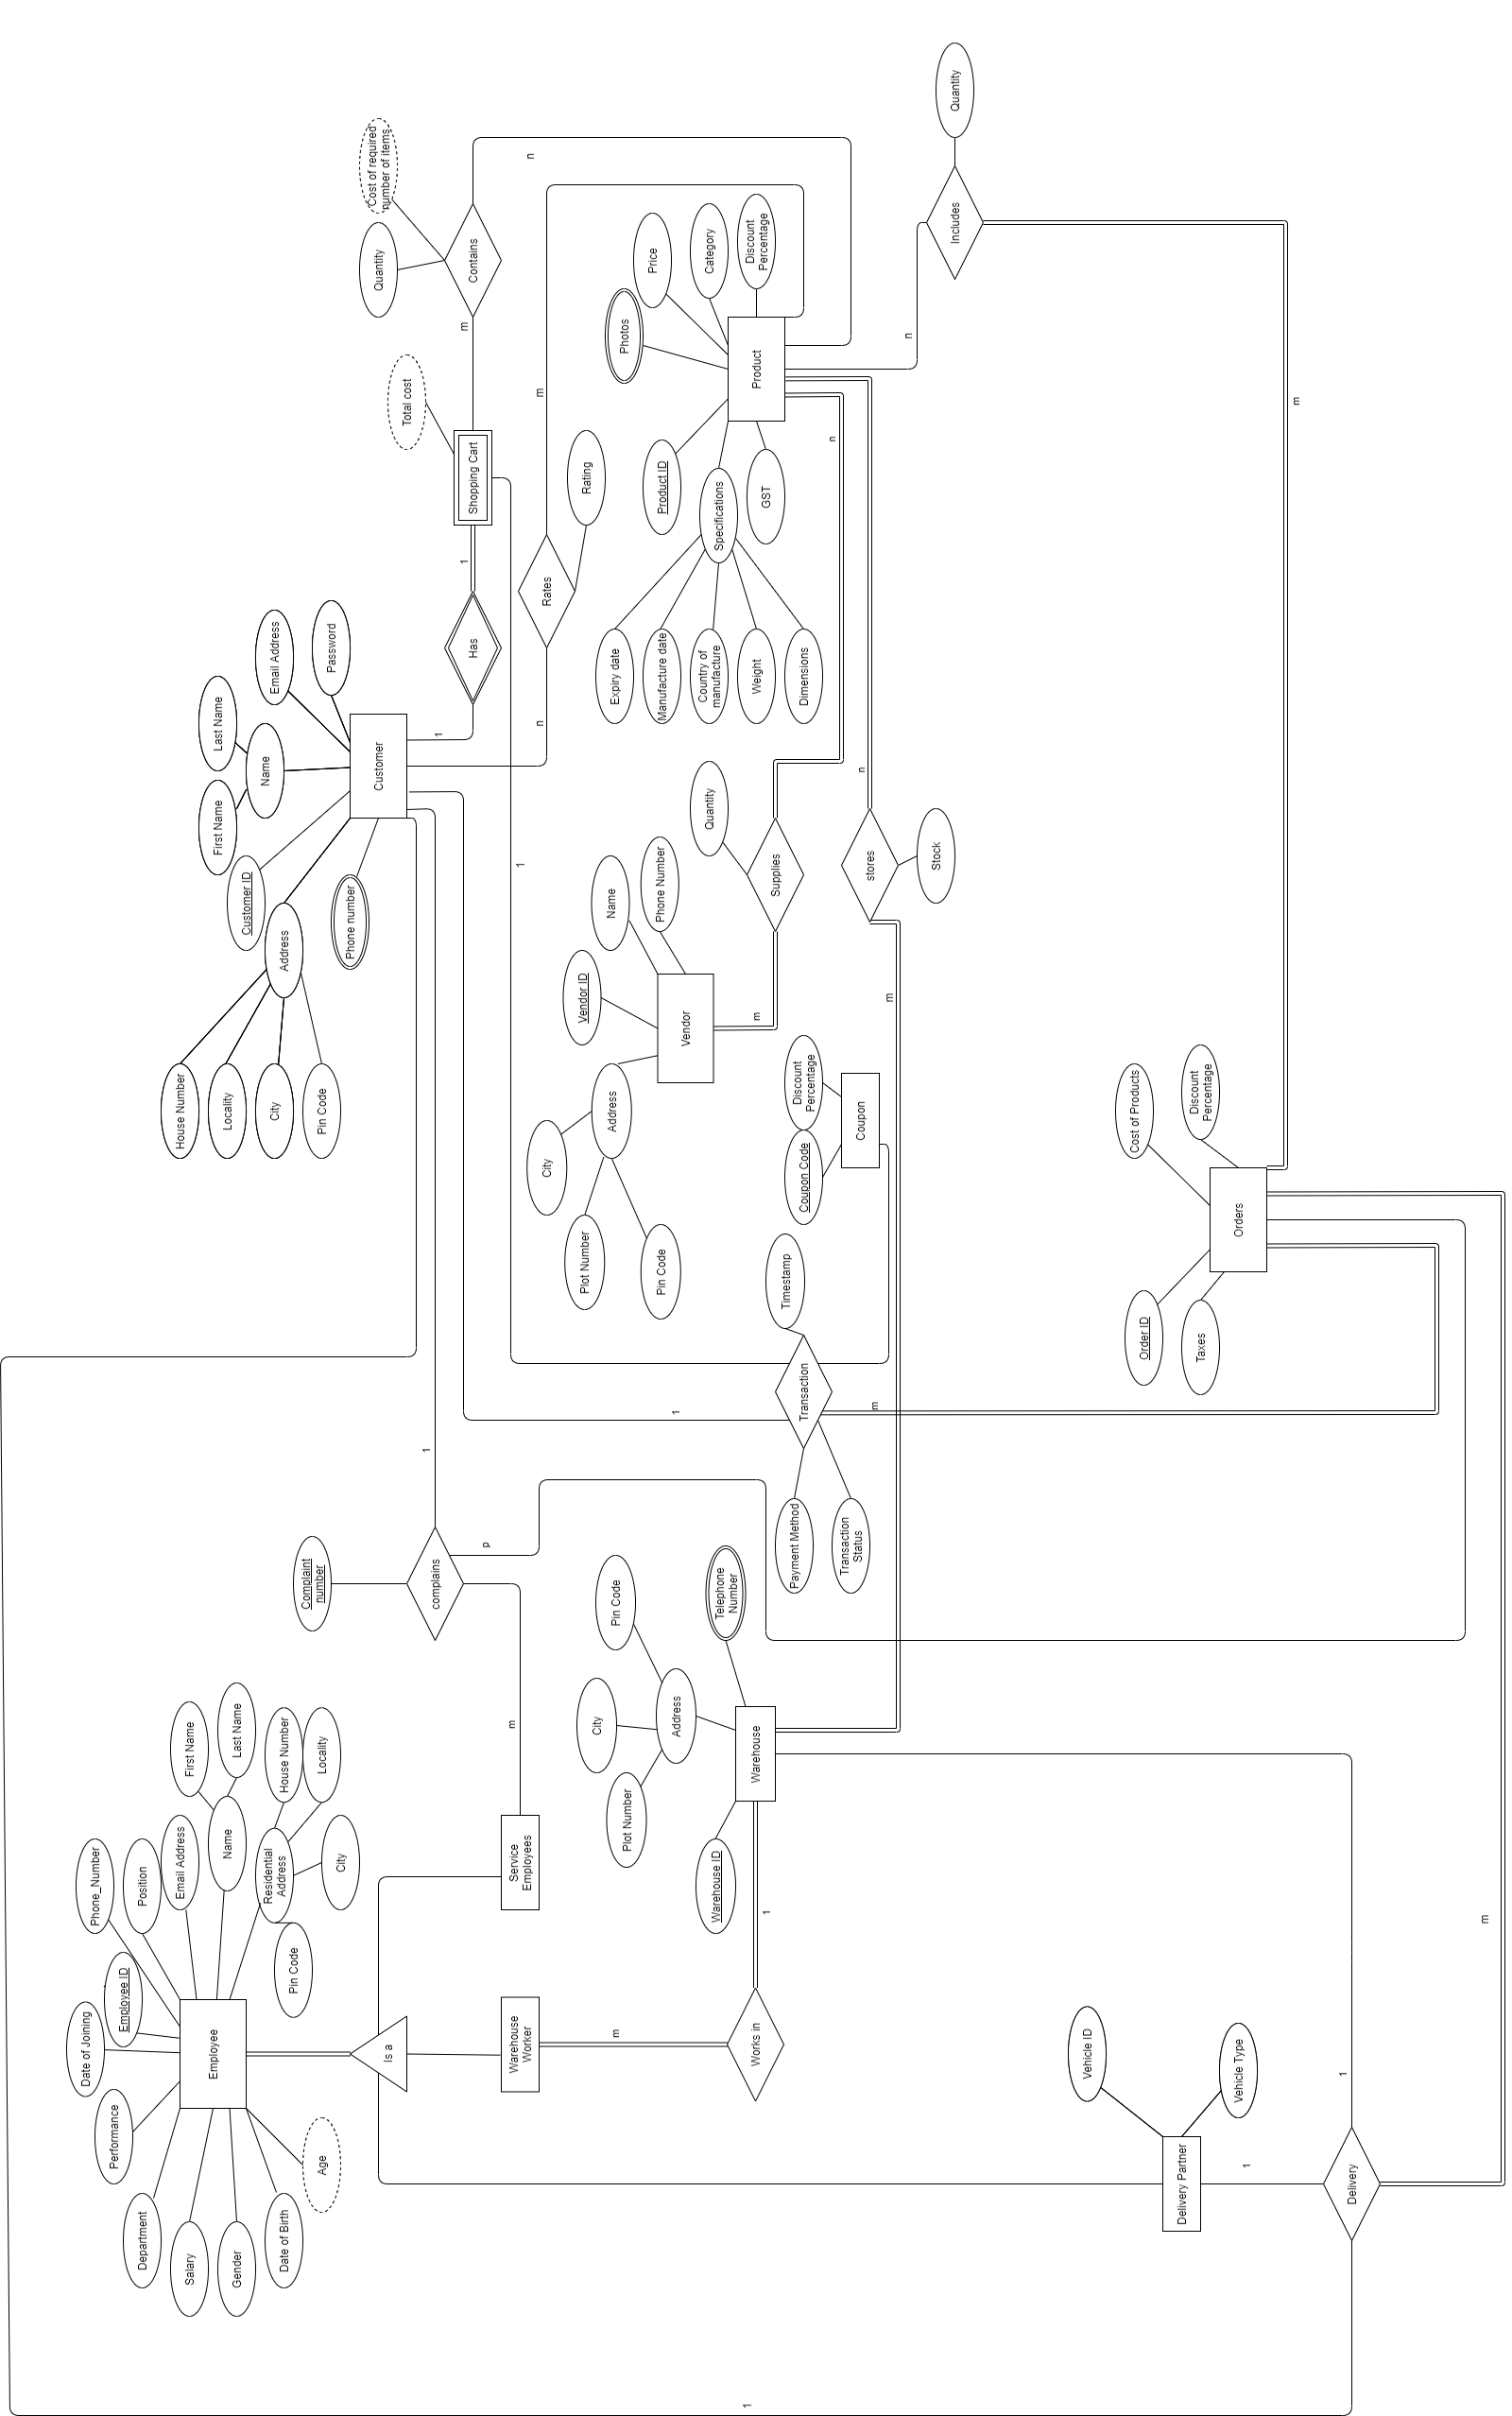
\includegraphics[width =0.85\textwidth]{Pictures/ER_Diagram.png}

\chapter{Relational Schema}
The ER diagram was reduced by noting multiplicities and the following tables for the relational schema resulted.

\begin{enumerate}
	\item Customer(\underline{customer ID}, )
	\item Product(\underline{product ID}, Price, Category, Discount Percentage, GST Percentage)
	\item Product Rating(\underline{Product ID, Customer ID}, Rating)
	\item Product Photo(\underline{Product ID, Product Photo})
	\item Vendor(\underline{Vendor ID}, First Name, Last Name, Plot Number, City, Pincode)
	\item Vendor Phone(\underline{Vendor ID, Phone Number})
	\item Warehouse(\underline{Warehouse ID}, Plot Number, City, Pincode)
	\item Warehouse Phone(\underline{Warehouse ID, Phone Number})
	\item Employee(\underline{Employee ID}, First name, Last name, Age, Salary, Gender, Department, Performance, Position, Date of Joining, Date of Birth, Email Address, House Number, Locality, City, Pincode, Phone Number)
	\item Delivery Partner(\underline{Employee ID}, Vehicle ID, Vehicle Type)
	\item Warehouse Worker(\underline{Employee ID})
	\item Service Employee (\underline{Employee ID})
	\item Orders(\underline{Order ID}, Total Price, Taxes, Total Discount Percentage)
	\item Coupon(\underline{Coupon Code}, Discount Percentage)
	\item Transaction(\underline{Order ID}, Payment Method, Transaction Status ,Transaction Time, Customer ID, Coupon code)\\ Here, Customer ID is referenced from Customer table and coupon code from Coupon table. Coupon code can be null, customer id cannot.
	\item Delivery (\underline{Order ID}, Employee ID, Customer ID, Warehouse ID) \\ Here Employee ID is taken from the Employee table if it belongs to Delivery Partner, Customer ID from Customer table, Warehouse ID from Warehouse table.
	\item Stores(\underline{Warehouse ID, Product ID}, Quantity)
	\item Supplies(\underline{Vendor ID, Product ID}, Quantity)
	\item Shopping Cart(\underline{Customer ID, Product ID}, Quantity)
	\item Complains(\underline{Complaint Number}, Customer ID, Order ID, Service Employee ID)\\ Here, Customer ID is taken from Customer table, Order ID from Orders table, Service Employee ID from Service Employees table.
	\item Order Products(\underline{Order ID, Product ID}, Quantity)

\end{enumerate}

\textbf{\underline{ Note}}: Employee has both fields of age and DOB. This is a redundancy on our part as the data entries were designed with age as an attribute. This may be eliminated in the final version depending on whether there is need or not (number of employees should be significantly lower than the number of customers).
\\
The SQL queries for creating the database, populating the database and the queries required are submitted under the names: 'database\_creation.sql', 'database\_population.sql' and 'queries.sql'.

\chapter{Contributions of Team Members}
\end{document}